\section[Metrology of the gradient magnetic field]
{Accuracy bound for gradient field estimation with atomic ensembles}
\thiswatermark{\put(1,-282){\color{l-grey}\rule{84pt}{88pt}}
\put(84,-282){\color{grey}\rule{410pt}{88pt}}}


\lettrine[lines=2, findent=3pt, nindent=0pt]{I}{n} this chapter, one of the most fundamental two-parameter estimation tasks in magnetometry is considered, namely gradient magnetometry.
We will add the gradient of the magnetic field as the second parameter beside the constant (homogeneous) part of the field.
While most works in magnetometry with a single ensemble focus only on the determination of the strength and direction of magnetic field, certain measurement schemes for the gradient have already been proposed and tested experimentally [XXX].
Some schemes use an imaging of the ensemble with a high spatial resolution, however, they do not count as single-ensemble methods in the sense we use this expression in our paper, since in this case not only collective observables are measured  \cite{Vengalattore2007,Zhou2010,Koschorreck2011}.
There is a method based on collective measurements of the spin length of a fully polarised ensemble \cite{Behbood2013}.
Finally, there is a scheme where they use as a prove state a many-body singlet states, which is described in Reference~\cite{UH13}.
This section provides precision bounds for that scheme, while expanding the quantum states considered to other interesting quantum states, including those that are not invariant under homogeneous fields.

The atoms will be distributed along the $OX$ axis, so $y=z=0$, and in principle they will be able to feel differences on the magnetic field at different points of the axis.
The magnetic field at the atoms will be given by a linear function on the position $x$
\begin{equation}
\bs{B}(x,0,0)=\bs{B}_0 +x \bs{B}_1 + O(x^2),
\end{equation}
where we will neglect the terms of order two or higher.
We will consider the magnetic field pointing along the $OZ$ direction direction only, $\bs{B}_0=B_0 \bs{k}$ and $\bs{B}_1=B_1\bs{k}$, where $\bs{k}$ is the unitary vector pointing on the $OZ$ direction.
For this configuration, due to the Maxwell equations, with no currents or changing electric fields, we have
\begin{align}
\nabla \cdotp \bs{B}&=0, \nonumber \\
\nabla \times \bs{B}&=\bs{0}.
\end{align}
This implies $\sum_{l=x,y,z} \partial_l B_l=0$ and $ \partial_m B_l - \partial_l B_m =0$ for $\forall l\ne m$, where $\partial_m\equiv \partial/\partial_m$ stands for the partial derivative over the variable $l$.
Thus, the spatial derivatives of the field components are not independent of each other.
However, in the case of a linear arranged particle ensemble only the derivative along the $OX$ axis has an influence on the quantum dynamics of the atoms.

% THIS IS NOT SO SIMPLE. CORRECT!
%The states of the ensembles are assumed to be permutationally invariant (PI),
%since the particles cannot be addressed individually.% anyway.

We will determine the precision bounds for estimation of the magnetic field gradient $B_1$ based on the quantum Fisher information (QFI) \cite{Paris2009,Braunstein1994,Holevo1982,Helstrom1976,Petz2002,Petz2008}.
We will show that for states insensitive to the homogeneous magnetic field, one can reduce the problem to a one-parameter estimation scenario.
Such states can arise in a single-ensemble scheme, however, it will be shown that for single-ensembles insensitive to the homogeneous field the Heisenberg limit cannot be reached.
Nevertheless, single-ensemble measurements have certain advantages since the spatial resolution can be higher and the experimental requirements are smaller since only a single ensemble must be prepared.

On the other hand, for states sensitive to the homogeneous field, the classical limit can be overcome only if the particle positions are highly correlated with each other.
Our calculations are generally valid for any measurement, thus they are relevant to many recent experiments \cite{Wasilewski2010,Eckert2006,Wildermuth2006, Wolfgramm2010,Koschorreck2011,Vengalattore2007,Zhou2010,Behbood2013}.
We note that in the case of the singlet, our precision bounds are saturated by the metrological scheme presented in Reference~\cite{Urizar-lanz2013}.

We can also connect our results to entanglement theory \cite{Werner1989,Horodecki2009,Guehne2009}.
We find that the shot-noise scaling cannot be surpassed with separable states, while the Heisenberg scaling can be reached with entangled states.
However, the shot-noise scaling can be surpassed only if the particle positions are correlated, which is the case if the particles attract each other.
Moreover, the case of two atomic ensembles, if the spin states of the ensembles are uncorrelated, can also be mapped to our model.
This evidently shows how shot-noise scaling can be surpassed with the two-ensemble scenario.

Next, we will present characteristics of our setup.
For simplicity, as well as following  recent experiments (e.g., Ref.~\cite{Koschorreck2011}), we will consider an ensemble of spin-$j$ particles placed in a one-dimensional setup, $x$ being the spatial coordinate.
Furthermore, we assume that we have that we have particles that behave classically with respect to their spatial state.
That is, they cannot be in a superposition of being in two different positions.
On the other hand, they have internal degrees of freedom, their spin, that is quantum. This is a very good description to many of the cold gas experiments.

Based on these considerations, we assume that the state is factorizable into a spatial and a spin part as
\be
\label{eq:separated-internal-and-external}
\rho=\rho_{{\rm x}}\otimes\rho_{{\rm s}},
\ee
and that the spatial part can be characterized as an incoherent mixture of point-like particles that can be written as
\be
  \label{eq:thermal-state}
  \rho_{\rm x}=\int d^N\bs{x}\, P_N(\bs{x}) \ket{\bs{x}}\bra{\bs{x}}.
\ee
Note that the spatial part is diagonal on the position eigenbasis, where the entry $x_n$ of $\bs{x} =(x_1,\dots,x_N)$ is the coordinate of the $n^{\rm th}$ particle, and $P_N(\bs{x})$ is the spatial probability distribution function of the atoms.
This model can be seen as that the density matrix of the spatial part of the state is diagonal on the position eigenbasis and it simplifies much the problem.
During the evolution of the state, correlations might arise between the two inner and spatial parts and the product form \eqref{eq:separated-internal-and-external} might be not valid to describe the evolution of the system.

We note that our method could be easily extended to the case of Bose-Einstein condensates, not considered in this paper. In that case, the spatial state of the particles would be a pure state, and we would have $\rho_{\rm x}=(\vert\Psi\rangle\langle\Psi\vert )^{\otimes N},$ where $\ket{\Psi}$ is a spatial single-particle state.

Although in our case the parameter to be estimated is $B_1$,
the time-evolution of the state is usually also affected by the second unknown
parameter, the homogeneous field $B_0$, which means that we generally have to
consider a two-parameter estimation problem.
The angular momentum of an individual atom is
coupled to the magnetic field, yielding the following
interaction term
\be
h^{(n)}=\gamma B_z^{(n)} \otimes j_z^{(n)},
\ee
where the operator $B_z^{(n)}=B_0+B_1x^{(n)}$ acts on
the spatial part of the Hilbert space.
%The
%individual atoms will interact with the magnetic field through
%a coupling with their angular
%momentum in the following way,
%\be
%h^{(n)}=\gamma B_z^{(n)} (x^{(n)}) \otimes j_z^{(n)},
%\ee
%where the magnetic field acts also as an operator because it depends on the
%position of each particle and it is no longer a constant, $B_z^{(n)}(x^{n})=B_0+B_1
%x^{(n)}$.
The sum  of all one particle interactions provide the total Hamiltonian
\be
\label{eq:Htot}
H = \gamma \sum_{n=1}^N B_z^{(n)} \otimes j_z^{(n)},
\ee
which will generate the time evolution of the atomic ensemble.

%Hamiltonians should evolve the system
%in time,
%\be
%\label{eq:Htot}
%H = \gamma \sum_{n=1}^N B_z^{(n)} \otimes j_z^{(n)},
%\ee
%Hence Eq.~\eqref{eq:Htot} is the total Hamiltonian of the system.

We will estimate the precision of $B_1$ based on a measurement
on the state after it passed through the dynamics
expressed by the unitary evolution operator $U=\exp(-i\frac{H}{\hbar}t)$,
where $t$ is the time spent by the system under the influence of the magnetic field.
Those type of unitary phase shift are the most easy ones to study with the quantum Fisher information, and this is the reason while we choose them to make the jump to the multi-parametric estimation problem.
The unitary operator can be rewritten in the following way
\be
\label{eq:unitary evolution with time and gamma encoded in b_0 and b_1}
U=e^{-i \lpar b_0 H_0 + b_1 H_1 \rpar},
\ee
where the $b_i=\gamma B_i t/\hbar$.
Here, the generator describing the effect of the homogeneous field is  given as
%the \emph{homogeneous phase shift} generator
%Hence, the two
%generators can be expressed as the
\be
\label{eq:homogeneous-generator}
H_0=\sum_{n=1}^N j_z^{(n)} = J_z,
\ee
%and the \emph{gradient phase shift} generator
 while the generator describing the effect of the gradient is
 %the \emph{gradient phase shift} generator
\be
\label{eq:gradient shift generator}
H_1=\sum_{n=1}^N x^{(n)}j_z^{(n)}.
\ee
As in Eq.~(\ref{eq:gradient shift generator}), we will usually omit %writing
$\otimes$ for simplicity,
%since it is clear that both operators $x^{(n)}$ and $j_z^{(n)}$
%belong to different tensor components of the physical Hilbert space;
and will use it only  if it is necessary to make our explanation clearer.

Note that the operators $H_{0}$ and $H_{1}$ commute with each other.
These two commuting dynamics are the two simplest in an atomic ensemble as
they are based on collective operators not requiring an individual access to
the particles.
%The Hamiltonian $H_{0}$ describes a rotation by a homogeneous
%magnetic field, while $H_{1}$ describes the action of a field gradient.

Note also that it is not necessarily
true that the operators we have to measure to estimate $b_0$ and $b_1$
commute with each other, which problem we will consider case by case.
The reason for that is that both operators to be measured
act on the same single atomic ensemble.
On the other hand, in schemes in which the gradient is calculated
based on measurements in two separate atomic ensembles or
different atoms in a chain, the measuring operators can always commute
with each other \cite{Wasilewski2010,Eckert2006,Zhang2014}.

The paper is organized as follows. In Sec.~\ref{sec:cramer-rao bounds}, the
basic concepts used in the paper are presented.
In Sec. III, we restrict our calculations to single PI atomic ensembles and we
develop some particular cases, such as the singlet spin state
or the totally polarised state. In Sec. IV, we discuss our results.

%%%%%%%%%%%%%%%%%%%%%%%%%%%%%
\subsection{Cram\'er-Rao precision bounds}
\label{sec:cramer-rao bounds}
%%%%%%%%%%%%%%%%%%%%%%%%%%%%%

%After explaining the basic concepts about the magnetic field and its
%interaction with the system,
In this section, we show how the Cram\'er-Rao bound and the QFI help us to obtain the precision bound that is valid for any measurement scenario.
We will discuss gradient magnetometry using quantum states that are insensitive to homogeneous fields, which is a single-parameter estimation task.
Then, we discuss the case of quantum states sensitive to homogeneous fields.
We show that the precision bound obtained does not change under spatial translation.
Since this is a two-parameter estimation task, we will introduce the two-parameter Cram\'er-Rao bound and the corresponding two-parameter QFI matrix, and we adapt those expressions to our problem.

For clarity we present our main tools inf subsequent paragraphs before going onto details for states that are not sensitive to the homogeneous field and states that they are.
The expression for quantum Fisher information that we use along this paper will be suitable for the transition to the multi-parameter problem\ie it is equivalent for the single parameter estimation problem still giving the chance to switch to the multi-parameter case.
For two arbitrary operators $A$ and $B$, it is written as follows
\be
  \label{eq:FAB}
  \qfi[\rho,A,B]:=2\sum_{k, k'}
  \frac{(\lambda_k-\lambda_{k'})^2}{\lambda_k+\lambda_{k'}}
  {A}_{k,k'}{B}_{k',k},
\ee
where the subscript for $A$ and $B$ stand for the matrix element on the eigenbasis of the initial state $\rho = \sum_k\lambda_k\ket{k}\bra{k}$.
If the two operators are the same, the usual form of the QFI on the literature can be recovered with only two arguments \cite{Paris2009,Braunstein1994,Holevo1982,Helstrom1976,Petz2002,Petz2008},
\be
  \qfi[\rho,A,A]:=\qfi[\rho,A]=2\sum_{k, k'}
  \frac{(\lambda_k-\lambda_{k'})^2}{\lambda_k+\lambda_{k'}}
  |{A}_{k,k'}|^2.
\ee
We mention that in our case the operators $A$ and $B$ will commute on all cases making the some computations easier.
We also make use of the fact that the QFI as written as in Eq.~(\ref{eq:FAB}) is linear on the second and last arguments,
\be
  \label{eq:qfi-linear-in-arguments}
  \qfi[rho, A, \sum_i b_i] = \sum_i \qfi[\rho,A,b_i]
\ee
together with $\qfi[\rho, A, B] = \qfi[\rho, B,A]$ so the statement holds.

Some more useful properties of the Eq.~(\ref{eq:FAB}).
It can be rewritten as follows,
\be
  \label{eq:QFI for two operators rewrited}
  \qfi[\rho, A, B] = 4 \expect{AB}
  - 8\sum_{k,k'}
  \tfrac{\lambda_k\lambda_{k'}}{\lambda_k+\lambda_{k'}}
  {A}_{k,k'}{B}_{k',k}.
\ee
This form leads to simple arguments on our derivations on following sections.
For pure states it simplifies to,
\be
  \label{eq:QFI_pure}
  \qfi[\ket{\psi},A,B]=4\l(\expect{AB}_{\psi}-\expect{A}_{\psi}\expect{B}_{\psi}\r).
\ee
Notice that we recover $\qfi[\rho,A]=4(\Delta A)^2$ as can be found in the literature for single parameter estimation with pure states \cite{Paris2009,Toth2013}.
Another important feature of the qFI in Eq.~(\ref{eq:FAB}) is that it is convex on the space of the states.
This property takes the following form,
\be
  \qfi[q\rho_1{+}(1{-}p)\rho_2]\leq
  p\qfi[\rho_1]{+}(1{-}p)\qfi[\rho_2],
\ee
where we omit in writing the arguments for the operators of the qFI for simplicity.

In the following subsections we show the general form for the precision bounds for states insensitive to the homogeneous fields and for states sensitive to them. We also show that both bounds are invariant under spatial translation of the system which makes the computing for particular cases much easier.

%%%%%%%%%%%%%%%%%%%%%%%%%%%%%
\subsubsection{Precision bound  for states insensitive to homogeneous fields:
Single-parameter dependence}
%%%%%%%%%%%%%%%%%%%%%%%%%%%%%

Let us consider quantum states that are  insensitive to the homogeneous field.
For these states,  $[\rho, H_0]=0$ and hence the evolved state is a function of a single unknown parameter, $b_1$.

For the unitary dynamics we consider, the QFI for single-parameter dependence can be expressed in terms of the eigendecomposition of the density matrix,
$\rho=\sum_{k} \lambda_k \ket{k}\bra{k}$, in the following way  \cite{Paris2009,Braunstein1994,Holevo1982,Helstrom1976,Petz2002,Petz2008},
\be
  \label{eq:general one parameter quantum fisher information}
  \qfi[\rho,H_1]=2\sum_{k, k'}
  \frac{(\lambda_k-\lambda_{k'})^2}{\lambda_k+\lambda_{k'}}
  |({H_1})_{k,k'}|^2.
  \ee
  And due to the Cram\'er-Rao formula gives us an upper
  bound for the precision
  \be
  \label{eq:one parameter precision bound}
  (\Delta b_1)^{-2}|_{\max} = \qfi[\rho,H_1].
\ee
Note that it is always possible to find a measurement that saturates the above precision bound.
Here, $\qfi[\rho,H_1]$ denotes the QFI that depends, in the case of unitary transformation of the form Eq.~\eqref{eq:unitary evolution with time and gamma encoded in b_0 and b_1}, on the state $\rho$ and on the generator of the evolution, $H_1$.

For the particular case on which the states has the form of Eqs.~(\ref{eq:separated state
internal and external}) and (\ref{eq:cold atomic ensemble state}) the Equation~(\ref{eq:general one parameter quantum fisher information}) can be simplified in the following way, see that we have to compute the matrix elements of $H_1$ but it is already diagonal on the spatial subspace.
Therefore the following holds for the matrix elements,
\be
  \begin{split}
    (H_1)_{\bs{x},k,\bs{y},k'}
    &=\bra{\bs{x},k}{H_1}\ket{\bs{y},k'}\\
    &=\bra{\bs{x},k}{\sum_{n=1}^N x^{(n)}j^{(n)}}\ket{\bs{y},k'}\\
    &=\delta(\bs{x}-\bs{y})\sum_{n=1}^N x_n\bra{k}{j^{(n)}}\ket{k'}.
  \end{split}
\ee
We will use the Dirac delta function to further simplify the Equation~(\ref{eq:general one parameter quantum fisher information}), for details of the simplification see the Appendix~\ref{ap:long-calc}.

For the last part of the proof on which we have to show how translated systems have unchanged the sensitivity over the gradient estimation, we use the Heisenberg picture on which the operators must be reversely transformed instead of the states.
Thus, we compute the transformation of $H_1$ in the following way,
\be
\begin{split}
\label{eq:shifted h1 generator}
U_d:H_1 \rightarrow H_1(d)
&=  U_d^{\dagger}H_1U^{\phantom\dagger}_d\\
&=\sum_{n=1}^N U_d^{\dagger}x^{(n)}U^{\phantom\dagger}_d  \otimes j_z^{(n)}\\
&=\sum_{n=1}^N (x^{(n)}-d)j_z^{(n)}\\
&=H_1-dH_0.
\end{split}
\ee
Hence, the new unitary evolution operator instead of Equation~(\ref{eq:unitary evolution with time and gamma encoded in b_0 and b_1}) will be
\be
%U=e^{-ib_1H_1}\,\rightarrow\,
U=e^{-i(b_0H_0+b_1 H_1(d))}=e^{-i((b_0-b_1d)H_0+b_1H_1)},
\ee
which for states insensitive to the homogeneous field, $[\rho, H_0]=0$, makes the transformation irrelevant.

With this, for states of the form Equations~(\ref{eq:separated-internal-and-external},\ref{eq:cold atomic ensemble state}) the following bound for the precision of the estimation of the gradient parameter $b_1$ holds,
\be
  \label{eq:bound-for-insensitive-and-thermal-state}
  (\Delta b_1)^{-2}|_{\max} = \sum_{n,m}^N \int d^N\bs{x}P_N(\bs{x})x_n x_m \qfi[\rho_{\rm s}, j_z^{(n)}, j_z^{(m)}],
\ee
where the integral results onto a two-point correlation function of the spatial state.

Moreover, such bound is translationally invariant\ie it remains the same after an arbitrary phase-shift of the form of $U_d=\exp(-i \bs{d} \cdot \bs{p}_{\rm x})$, where $\cdot$ denotes scalar product, $\bs{d}$ is a $n$-length vector of all elements equal to the phase-shift $d$ and $\bs{p}_{\rm x}$ is the vector that collects all the single particle linear momentum operators, $p_{\rm x}^{(n)}$.

%%%%%%%%%%%%%%%%%%%%%%%%%%%%
\subsubsection{Precision bound for states sensitive to homogeneous fields:
Two-parameter dependence}
%%%%%%%%%%%%%%%%%%%%%%%%%%%%

In order to obtain the precision bound for states sensitive to the
homogeneous field, one has to consider the effect on the state of a second
unknown parameter, in this case $b_0$.
The homogeneous field will rotate all the spins in the same way,
while the field gradient rotates the spins
differently depending on the position of the particles.
Now, instead to the Cram\'er-Rao bound  \eqref{eq:one parameter precision bound},
we have a matrix inequality \cite{Paris2009}.
%The Cram\'er-Rao bound turns into a matrix inequality of a similar form as Eq.
%\eqref{eq:one parameter precision bound}, namely
% \be
% \label{eq:matrix cramer-rao equation}
% \textbf{Cov}[b_0,b_1]\geq \bs{\mathcal{F}}_{\text{Q}}^{-1},
% \ee
% where the covariance matrix elements are defined as
% $\textbf{\cov}_{ij}[b_0,b_1]=\expect{b_ib_j}-\expect{b_i}\expect{b_j}.$
We have the QFI matrix $\bs{\mathcal{F}}_{\text{Q}}$ on one hand, which depends on $\rho$ and the two generators $H_0$ and $H_1$, and the covariance matrix from we are only interested on the variance of the gradient parameter, $(\Delta b_1)^2$ \cite{Paris2009}.
Just to record, $H_0$ and $H_1$ are Hermitian operators and commute with each other and thus the QFI matrix elements are computed as $\mathbfcal{F}_{ij}\equiv \qfi[\rho, H_i, H_j],$ following the definition \eqref{eq:FAB}.

In the two-parameter estimation problem, ${\mathbfcal{F}}$ is a $2 \times 2$ matrix and the precision bound for the estimation of the gradient is the following,
\be
\label{eq:precision bound for b1 in terms of QFI matrix elements}
(\Delta b_1)^{-2}\leq \mathbfcal{F}_{11}-\frac{\mathbfcal{F}_{01}\mathbfcal{F}_{10}}{\mathbfcal{F}_{00}},
\ee
where $\mathbfcal{F}_{ij}$ denotes the QFI matrix elements.
One must estimate both parameters in most cases since the precision of one depends on the other.
The bound is interpreted slightly different from the one-parameter Cram\'er-Rao bound.
In order to be able to saturate the bound the measurements for estimating the two parameters must compatible \cite{Paris2009}.


To compute the bound (\ref{eq:bound-for-insensitive-and-thermal-state}) we need to consider the matrix elements of QFI one by one.
First of all, we compute $\mathbfcal{F}_{11}$ that without assuming anything else has the same form as Equation~(\ref{eq:bound-for-insensitive-and-thermal-state})
\be
  \mathbfcal{F}_{11}=\sum_{n,m}^N \int d^N\bs{x}P_N(\bs{x})x_n x_m \qfi[\rho_{\rm s}, j_z^{(n)}, j_z^{(m)}].
\ee
Second, the most trivial matrix element is $\mathbfcal{F}_{00}$ which is a function of the internal state $\rho_{\rm s}$.
To compute it one must notice that
\be
\begin{split}
  (H_0)_{\bs{x},k,\bs{y},k'}
  &=\bra{\bs{x},k}{H_0}\ket{\bs{y},k'}\\
  &=\bra{\bs{x},k}{J_z}\ket{\bs{y},k'}\\
  &=\delta(\bs{x}-\bs{y})(H_0)_{k,k'}.
\end{split}
\ee
And with this it is straightforward to obtain
\be
  \mathbfcal{F}_{00} = \qfi[\rho_{\rm s}, J_z].
\ee
Note that this is not a function of the whole state but only of the internal $\rho_{\rm s}$ state.
Finally, we compute both $\mathbfcal{F}_{01}$ and $\mathbfcal{F}_{10}$.
To compute this, one may notice first that both matrix elements are equal, $\mathbfcal{F}_{01}=\mathbfcal{F}_{01}$.
Therefore we have to compute only one of them.
The computation follows,
\be
  \mathbfcal{F}_{01} = \sum_{n=1}^N \int d^N\bs{x}P_N(\bs{x})x_n\qfi[\rho_{\rm s}, j_z^{(n)},J_z].
\ee
With those results the Equation~(\ref{eq:bound-for-sensitive-and-thermal-state}) follows.
For further details see Appendix~\ref{ap:long-calc}.

For the last part of the proof, we need to show that his bound is invariant under translations as it is the Equation~(\ref{eq:bound-for-insensitive-and-thermal-state}).
With this aim, using the linearity of the last two arguments of $\qfi[\rho, A, B]$, Eq.~(\ref{eq:qfi-linear-in-arguments}), the fact that $H_0$ remains unchanged on the Heisenberg picture and using the shifted $H_1$ operator, Eq.~(\ref{eq:shifted h1 generator}), we have that
\begin{align}
  \mathbfcal{F}_{00}(d)&=\qfi[\rho, H_0(d)] = \qfi[\rho, H_0],\\
  \mathbfcal{F}_{01}(d)&=\qfi[\rho, H_0(d), H_1(d)]\nonumber\\
        &= \qfi[\rho, H_0,H_1-dH_0] = \mathbfcal{F}_{01}-d\mathbfcal{F}_{00},\\
  \mathbfcal{F}_{11}(d)&=\qfi[\rho, H_1(d), H_1(d)]\nonumber\\
        &=\qfi[\rho, H_1-dH_0,H_1-dH_0]\nonumber\\
        &=\mathbfcal{F}_{11}-2d\mathbfcal{F}_{01}+d^2\mathbfcal{F}_{00}.
\end{align}
Simple algebra shows that the bound for a displaced system is the same bound as is it would not be displaced,
\be
\begin{split}
  (\Delta b_1)^{-2}\leq\,&\mathbfcal{F}_{11}(d)-\frac{(\mathbfcal{F}_{01}(d))^2}{\mathbfcal{F}_{00}}\\
  =\,& \mathbfcal{F}_{11}-2d\mathbfcal{F}_{01}+d^2\mathbfcal{F}_{00}\\
  &-\frac{\mathbfcal{F}_{01}^2-2d \mathbfcal{F}_{01}\mathbfcal{F}_{00}+d^2\mathbfcal{F}_{00}^2}{\mathbfcal{F}_{00}}\\
  =\,& \mathbfcal{F}_{11}-\frac{\mathbfcal{F}_{01}^2}{\mathbfcal{F}_{00}}.
\end{split}
\ee
Hence, the Observation~XXX holds.

For states of the form Equations~(\ref{eq:separated-internal-and-external},~\ref{eq:thermal-state}), the expression to compute the precision precision bound takes the following form,
\be
\label{eq:bound-for-sensitive-and-thermal-state}
\begin{split}
  (\Delta b_1)^{-2}\leq& \sum_{n,m}^N \int d^N\bs{x}P_n(\bs{x})x_nx_m \qfi[\rho_{\rm s}, j_z^{(n)}, j_z^{(m)}]\\
  &- \frac{\l(\sum_{n=1}^N\int d^N\bs{x}P_n(\bs{x})x_n \qfi[\rho_{\rm s}, j_z^{(n)},J_z]\r)^2}{\qfi[\rho_{\rm s}, J_z]}.
\end{split}
\ee
Despite it seems to be complicated, this equation is easily computed for the most common cases such as trapped-ions, cold atomic ensembles the like.
This bound as well as Equation~(\ref{eq:bound-for-insensitive-and-thermal-state}) is invariant under spatial translations of the system.

This observations make the computation of the next sections easier since the now we can place the system arbitrarily wherever we choose.
It also allows us to place the origin of our coordinate system where the magnetic field is null.
So, the linear magnetic field can be written as $\bs{B}(x)= xB_1\bs{k}$ where $\bs{k}$ is the unitary vector pointing on the $OZ$ direction perpendicular to $OX$ and $OY$, making the estimation of the homogenous field irrelevant to compute the precision of the gradient parameter $b_1$.
Despite the redundant arguments used before, the discourse we have had on the preceding section has a vital importance to understand properly the gradient metrology on this context.


%%%%%%%%%%%%%%%%%%%%%%%
\subsection{Ion chains and two separated ensembles for magnetometry}
\label{sec:twin cloud systems}
%%%%%%%%%%%%%%%%%%%%%%%

Despite the powerfulness of our tools it is always nice to start with simple but concise examples to see how the results developed on the previous chapter behave.
For this goal we choose two state-of-the-art systems for the external states which a priori we know that behave well under the gradient interferometry.

\begin{figure}[htp]
\begin{center}
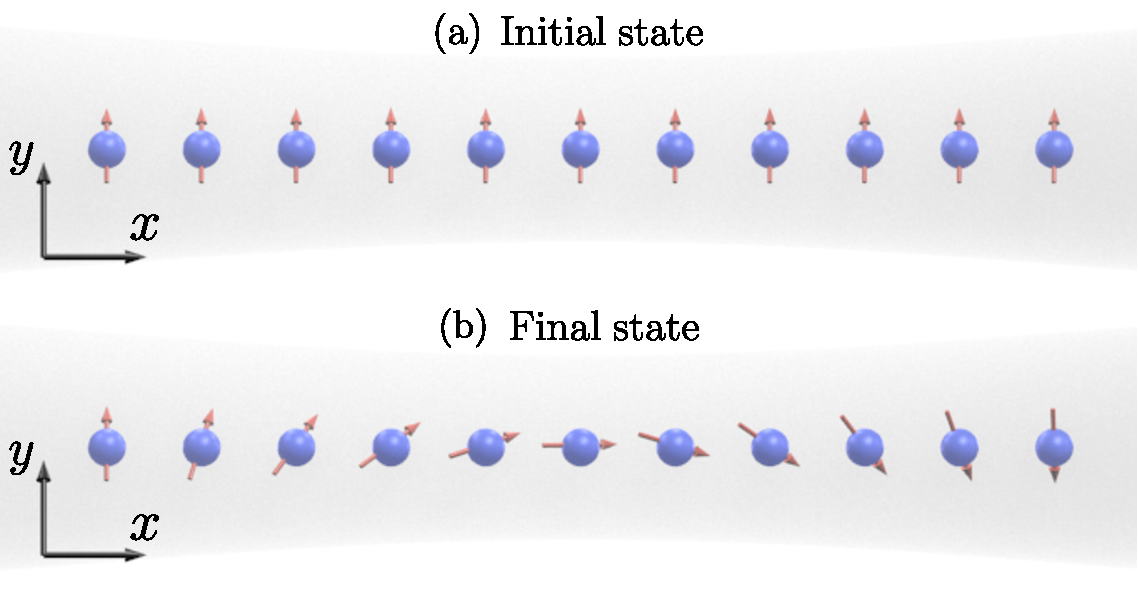
\includegraphics[width=244pt]{img/tp-density.pdf}
\caption{A one-dimensional chain of spin-$j$ atoms (blue
circles) confined in a potential (grey area).
(a) The ensemble is initially totally polarised along a
perpendicular direction of the magnetic field $B_z$ and the direction of the chain $OX$.
The internal state can be written as $\ket{j}_{y}^{\otimes N}$, the number represents $m_y$ the eigenvalue of the one particle operator $j_y^{(n)}$.
(b) One can see how the gradient field affects with a varying field strength the different spins when they are placed in different positions. }
\label{fig:ionchain-evolution}
\end{center}
\end{figure}

The first spatial state will be given by $N$ distinguishable ions all placed to a constant distance from the neighbor constituents on a single dimensional configuration\ie an ion-chain [Sanah's paper], see Figure~\ref{fig:ionchain-evolution}.
We have that for that matter the PDF describing the system is
\be
  P_N(\bs{x})=\prod_{n=1}^N \delta(x_n-na).
\ee

With this at hand we compute the single point averages and the two point averages corresponding to the ion-chain.
For the single point average we have that
\be
  \int d^N\bs{x}P_N(\bs{x}) x_n = na,
\ee
and for the two point average we have the following,
\be
  \int d^N\bs{x}P_N(\bs{x}) x_nx_m = nma^2.
\ee


We are going to compute  the precision bound when the internal state is a product state of all particles pointing onto $OY$ direction, $\ket{j}_y^{\otimes N}$, which is a state sensitive to the homogeneous field, so we have
\be
\label{eq:result-for-chain-without-sigma}
\begin{split}
  (\Delta b_1)^{-2}\leq \,&\sum_{n,m}^Nnma^2\qfi[\ket{j}_y^{\otimes N}, j_z^{(n)},j_z^{(m)}]\\
  &-\frac{\l(\sum_{n=1}^N a n \qfi[\ket{j}_y^{\otimes N}, j_z^{(n)},J_z]\r)^2}{\qfi[\ket{j}_y^{\otimes N}, J_z,J_z]}\\
  =\,& a^2 \l\{ \sum_{n=1}^N 2jn^2 - \frac{(\sum_{n=1}^N 2jn)^2}{2jN}\r\}\\
  =\,& 2a^2j N \frac{N^2 -1}{12},
\end{split}
\ee
where we have used the $\qfi[\ket{\psi},A,B]=4(\expect{AB}-\expect{A}\expect{B})$ identity to compute the calculations.

Despite that Equation~(\ref{eq:result-for-chain-without-sigma}) is a third order function of the particle number $N$ and that it seems to overcome the ultimate limit HL, on should notice that the length of the chain increases as we introduce more particles into the system.
This result, without normalisation, has the potential to confuse and cause false positives even with separable states \cite{Zhao2014}!
To solve this one can normalize the distance between the atoms or simply use some measure of spatial width of the complete system.
In our case we decide to use on all results the standard deviation of the averaged particle position as the length measure.
It is computed as follows,
\begin{align}
  \label{eq:mean}
  \mu &= \int d^N\bs{x}P_N(\bs{x}) \frac{\sum_{n=1}^N x_n}{N} \\
  \label{eq:variance}
  \sigma^2 &= \int d^N\bs{x}P_N(\bs{x}) \frac{\sum_{n=1}^N x_n^2}{N} - \mu^2\\
  \label{eq:variance-chain}
  \sigma_{\text{ch}}^2 &= a^2\frac{N^2-1}{12}.
\end{align}
It turns out that this exactly coincides with a factor we have on Equation~(\ref{eq:result-for-chain-without-sigma}).
Substituting this onto the result the proof concludes.

For ion-chains where their constituents are separated by a constant distance and where the spin-state $\rho_{\rm s}$ is the totally polarised state along a perpendicular direction of both the field and the chain direction, in this case $OY$, the precision bound is given by the following formula,
\be
  (\Delta b_1)^{-2}\leq 2\sigma_{\text{ch}}^2jN,
\ee
where $\sigma_{\text{ch}}$ denotes the standard deviation of whole position spots on which the particles rest, $j$ is the spin-number of each particle and $N$ is the particle-number.

We continue this illustrative example with the state-of-the-art double-well spatial state.
We also will use an internal state that with the maximal QFI so the reader gets familiar with our approach and sees how the best state to measure the gradient parameter looks like on our framework.

The spatial part is described by the following PDF where half of the particles are in one-well and the rest in the other, placed both positions at a distance of $a$ from the origin,
\be
  \label{eq:double-well-spatial-pdf}
  P_N(\bs{x})=\prod_{n=1}^N \delta(x_n + (-1)^n a),
\ee
where the "odd" particles go to the "right" and the "even" particles to the "left".
With this we are able to compute the single-point and two-point correlation functions as,
\begin{align}
  \int d^N\bs{x}P_N(\bs{x})x_n &= (-1)^{n+1}a,\\
  \label{eq:two-point-function-double-well}
  \int d^N\bs{x}P_N(\bs{x})x_nx_m &= (-1)^{n+m}a^2.
\end{align}

The state $\ket{\psi}$ is insensitive to the homogeneous field so we have that
\be
\begin{split}
  (\Delta b_1)^{-2}|_{\max} &= \sum_{n,m}^N (-1)^{n+m} a^2 \qfi[\ket{\psi}, j_z^{(n)}, j_z^{(m)}]\\
  &= a^2\sum_{n,m}^N (-1)^{n+m} 4 (-1)^{n+m} j^2\\
  &= 4 a^2 j^2 N^2,
\end{split}
\ee
where we have used the definition for pure states of QFI, $4(\expect{j_z^{(n)}j_z^{(m)}}-\expect{j_z^{(n)}}\expect{j_z^{(m)}})$.

On the other hand if we compute now the standard deviation as we did before for the case of the chain, Eqs.~(\ref{eq:mean}-\ref{eq:variance-chain}), we have that in this case $\mu=0$ and the standard deviation
\be
  \sigma_{\text{dw}}^2 = \int d^N\bs{x}P_N(\bs{x})=a^2,
\ee
with which the proof follows.
Before concluding the proof we want to show another more usual approach to the same problem.

It is as follows, given that the QFI is convex on states and having already fixed the external spatial state to be Equation~(\ref{eq:double-well-spatial-pdf}), the inner state that maximises the QFI is the one that maximises $(\Delta H_1)^2$.
In this case, taking into account the particle locations and that we have zero magnetic field at the origin,
\be
  H_{1,\text{eff}} = b_1a(\mtxid_{\text{od}}\otimes J_{z,\text{ev}}-J_{z,\text{od}}\otimes \mtxid_{\text{ev}}),
\ee
where we write the effective Hamiltonian that the particles feel and "od" and "ev" stand for odd and even particle index respectively.
From here it is easy to show that the state maximising such variance is the following,
\be
  \ket{\psi} = \frac{1}{\sqrt{2}}(\ket{0\cdots 0}_{\text{od}}\otimes\ket{1\cdots 1}_{\text{ev}}+\ket{1\cdots 1}_{\text{od}}\otimes\ket{0\cdots 0}_{\text{ev}}),
\ee
which is equivalent to the state in Equation~(\ref{eq:best-state}).
This proofs that we have use the right state, and with this we can compute the QFI as in the literature as $\qfi[\ket{\psi}, H_1] = 4(\Delta H_1)^2 = 4a^2j^2N^2$.
With this we finally conclude the proof.

The maximally entangled internal state that maximized the QFI too is
\be
  \label{eq:best-state}
  \ket{\psi}=\tfrac{1}{\sqrt{2}}(\ket{0101\cdots01}+\ket{1010\cdots10}).
\ee
Notice that this is a coherent state of all particles on the left "up" and all on the right "down" plus all on the left "down" and all on the right "up".
We will choose without loosing of generality the particles to be spin-$j$ particles.
For this state insensitive to the homogeneous field and in the double-well spatial configuration, Eq.~(\ref{eq:double-well-spatial-pdf}), the maximal achievable precision is
\be
  (\Delta b_1)^{-2}|_{\max} = 4 \sigma_{\text{dw}}^2 j^2N^2
\ee

In this section we have shown to the reader how one should handle the spatial width of the system for classifying it for gradient metrology as well as a state-of-the-art system on which the Heisenberg limit is achieved. Moreover, we have sown how to use the tools developed on previous section to compute simple bounds. In the next section we will focus on single cold-atoms ensembles since the play an important role on todays quantum technology and experiments and many groups are trying to realize them whit great success but with few theoretical support from our point of view.

%%%%%%%%%%%%%%%%%%%%%%%%%%%%
\subsection{Magnetometry with an atomic ensemble}
\label{sec:single cloud systems}
%%%%%%%%%%%%%%%%%%%%%%%%%%%%

In this section, we discuss magnetometry with a single
atomic ensemble in a more deep way than in the previous section.
For that, we present precision bounds for
the estimation of the magnetic field gradient, for
states that are insensitive to the homogeneous field.
We also present precision bounds for states that are sensitive to the
the homogeneous field.
We consider a one-dimensional cloud of spin-$j$ atoms
placed in a one dimensional trap, which is elongated
in the  $x-$direction.
The magnetic field points in the  $z-$direction,
and has a constant gradient along the $x-$direction.
The setup is depicted
in Fig.~\ref{fig:single cloud particle density under the magnetic gradient field}.
In the last part of this section, we calculate precision bounds for the
gradient estimation for some important multi-particle quantum states,
for instance, Dicke states or
Greenberger-Horne-Zeilinger (GHZ) states \cite{Greenberger1990}.
%In this section, we will consider Permutationally Invariant (PI) states for the
%single-cloud case.
Note that all these states are permutationally invariant (PI), since we
assume a PI procedure to prepare the states.

%%%%%%%%%%%%%%%%%%%%%%%%%%%
\subsubsection{Precision bound for an atomic ensemble}
%%%%%%%%%%%%%%%%%%%%%%%%%%%

An atomic ensemble is defined as a finite number of atoms where
they cannot be labeled individually.
Thus, the initial quantum state is assumed to be PI.
Hence apart from $\rho_{\rm s}$, the probability distribution function
$P_N(\bs{x})$, appearing in Equation~(\ref{eq:therma-state}),
must also be PI.
The permutational invariance of $P_N(\bs{x})$ implies that
\be
\label{eq:pi-for-pdf}
P_N(\bs{x})=\tfrac{1}{N!}\sum_{k}\Pi_k [P_N(\bs{x})],
\ee
where the summation is over all the possible permutations
of the variables $x_n$ denoted by
$\Pi_k.$
%changes the order of the $N$ variables
%according to such permutation $s$, and the sum is extended to all the possible
%permutations in the set of all the possible permutations for $N$
%entities $\Sigma_N$.

As we have shown on Observations~XXX and XXX, the precision bound is invariant under translations on the spatial Hilbert space.
This allows us to place the "center of mass" of the system at the origin of the coordinates.
With this simplifying assumptions the single-point average of the whole ensemble is
\be
\label{eq:system-at-origin-single-ensemble}
\mu = \int d^N\bs{x}P_N(\bs{x})x_n=0,
\ee
where we used the PI nature of $P_n(\bs{x})$ to eliminate the sum and the $N$ from the Equation~(\ref{eq:mean}).
We will do the same with the second moments appearing on the variance, Eq.~(\ref{eq:variance}).
%, Obs.~\ref{obs:translationally invariance of one parameter cr bound} and
%\ref{obs:invariance under translation for SH states}.
Because of this, the size of the system can be related with the single variable, $x_n$, variance
\be
\label{eq:sigma definition for the pdf}
\sigma^2=\int P_N(\bs{x})x_n^2\,d^N\bs{x},
\ee
for any $n$, which is simplified due to the fact that the system is placed at the origin.
In the same way, and due again to the PI nature of $P_N(\bs{x})$ we write the covariance of two particle positions as
\be
\label{eq:eta definition for the pdf}
\eta=\int P_N(\bs{x})x_nx_m \, d^N\bs{x}
\ee
for any $n\neq m$.
With this we have characterised all two-points correlations that potentially will appear on our calculations.
An interesting property of the covariance of this type is that it is a value bounded from below and from above by the variance itself and the particle number $N$ in the following way,
\be
  \frac{-\sigma^2}{N-1}\leq \eta\leq \sigma^2.
\ee
So it cannot contribute for a better scaling on the precision than since it scales as much as $\sigma^2$ with the particle number.
Notice that the lower bound scales worse.

First of all we show an important property of states insensitive to the homogeneous field and we do so using the fact that the QFI for the homogeneous field generator\ie $J_z$, on those states is zero, $\qfi[\rho,J_z]=0$.
The identity follows,
\be
\begin{split}
  \label{eq:qfi-identity-insensitive}
  \qfi[\rho, J_z] & = 0\\
  \sum_{n,m}^N \qfi[\rho,j_z^{(n)},j_z^{(m)}] & = 0\\
  \sum_{n=1}^N \qfi[\rho, j_z^{(n)}] & = -\sum_{n\neq m}^N \qfi[\rho,j_z^{(n)},j_z^{(m)}]
\end{split}
\ee
where we use the linearity on the second and third arguments of $\qfi[\rho, \cdot, \cdot]$ to jump to the second line and subsequently the last line follows.

From the definition of the QFI for states insensitive to the homogeneous field, Eq.~(\ref{eq:bound-for-insensitive-and-thermal-state}), we compute the bound for single ensembles in the following way,
\be
\begin{split}
  (\Delta b_1)^{-2}|_{\max} &= \sum_{n,m}^N \int d^N\bs{x}P_N(\bs{x})x_n x_m \qfi[\rho_{\rm s}, j_z^{(n)}, j_z^{(m)}]\\
  &=\sum_{n=1}^N \sigma^2 \qfi[\rho,j_z^{(n)}] + \sum_{n\neq m}^N \eta \qfi[\rho,j_z^{(n)},j_z^{(m)}].
\end{split}
\ee
Together with Equation~(\ref{eq:qfi-identity-insensitive}) the Observation~\ref{obs:bound-insensitive-single-ensemble} follows.

The precision is bounded from below for a single atomic ensemble
insensitive to homogeneous field with the following quantity
\be
\label{eq:precision bound for single-cloud systems IH}
(\Delta b_1)^{-2}|_{\max} = (\sigma^2-\eta) \sum_{n=1}^{N} \qfi[\rho_{\rm
s},j_z^{(n)}].
\ee
The bound in Eq.~\eqref{eq:precision bound for single-cloud systems IH}
can be saturated by an optimal measurement.
Nevertheless, it is worth to notice that it cannot surpass the
shot-noise scaling, $\sim N$, because $\qfi[\rho_{\rm
s},j_z^{(n)}]$, the QFI for the single-particle operator $j_z^{(n)}$,
cannot be larger than $j^2$.

First of all, notice that the second term appearing on Equation~(\ref{eq:bound-for-sensitive-and-thermal-state}) is proportional to the single-point average $\int d^N\bs{x}P_N(\bs{x})x_n$ which by definition is the same for any $x_n$ and by decision is chosen to be zero, since we placed the system at the origin.
So, we only have to compute the first term of the Equation~(\ref{eq:bound-for-sensitive-and-thermal-state}),
\be
\begin{split}
  (\Delta b_1)^{-2}\leq& \sum_{n,m}^N \int d^N\bs{x}P_n(\bs{x})x_nx_m \qfi[\rho_{\rm s}, j_z^{(n)}, j_z^{(m)}]\\
  =& \sum_{n=1}^N \sigma^2 \qfi[\rho,j_z^{(n)}] + \sum_{n\neq m}^N \eta \qfi[\rho,j_z^{(n)},j_z^{(m)}]\\
  =&(\sigma^2- \eta)\sum_{n=1}^N  \qfi[\rho,j_z^{(n)}] + \eta\sum_{n, m}^N  \qfi[\rho,j_z^{(n)},j_z^{(m)}],
\end{split}
\ee
where we add to the last term $\eta\sum_{n=1}^N \qfi[\rho,j_z^{(n)}]$ and subtract it from the first term.
From this, using the fact that the QFI is linear on the second and third arguments again, the proof holds.
% First, we have that for states that are sensitive to homogeneous fields,
% we have to compute the QFI matrix elements,
% Eqs.~(\ref{eq:qfi matrix element 11 point like atoms}~--~\ref{eq:qfi
% matrix element 00 point like atoms}).
% Without loss of generality, let us assume again that the origin
% of the coordinate system is at the mean of the particle positions, leading to
% Eq.~\eqref{eq:exp0}.
%One can note that if the state is centered around the origin and is PI,
%then
% This assumption, based on Eq.~\eqref{eq:qfi matrix element 01 point like atoms}
% implies $F_{01} =0.$ Hence, the precision bound for
% $b_1$, Eq.~\eqref{eq:precision bound for b1 in terms of QFI matrix elements}, is
% written in the following way
% \bea
% \label{eq:precision bound for SH PI as fisher of H1 H1}
% &&{\hskip-0.5cm}(\Delta b_1)^{-2}\leq F_{11}=\nonumber\\
% &&=\sum_{n,m}^{N}\qfi[\rho_{\rm s},j_z^{(n)},j_z^{(m)}]
% \int d^N\bs{x}\, P_N(\bs{x})x_nx_m.
% \eea
% Note that the precision bound unveiled above is the same as in the case of the
% precision bound for states that are insensitive to homogeneous given in
% Eq.~\eqref{eq:one parameter precision bound}, but in this case
% $\qfi[\rho_{\rm s},J_z]$ is different from zero.
%
% Next, we will express the right-hand side of
% Eq.~\eqref{eq:precision bound for SH PI as fisher of H1 H1}
% in a form that contains the $\sigma^2$ and $\eta,$
% helping us to understand how the bound scales with $N.$
% For that we will use Eq.~(\ref{eq:qfi matrix
% element 11 point like atoms}).
% After separating the the terms in the double sum in Eq.~(\ref{eq:qfi matrix
% element 11 point like atoms}) to a sum for which the particle indexes are equal
% with each other and to a sum for which they are not equal,
% using the definitions
% Eq.~(\ref{eq:sigma definition for the pdf},
% \ref{eq:eta definition for the pdf}),
% we arrive at the following expression,
% \be
% \label{eq: gradient fisher information}
% F_{11}
% =\sigma^2
% \sum_{n=1}^N
% \qfi[\rho_{\rm s},j_z^{(n)}]
% + \eta
% \sum_{n \neq m}^N
% \qfi[\rho_{\rm s},j_z^{(n)},j_z^{(m)}].
% %=N (\sigma^2-\eta)\qfi[\rho_{\rm
% %s},j_z^{(1)},j_z^{(1)}]+\eta \qfi[\rho_{\rm s},J_z,J_z].
% \ee
% After using the facts that the following identity holds for any state,
% $\qfi[\rho_{\rm s}, J_z]=N\qfi[\rho_{\rm
% s},j_z^{(1)}]+N(N-1)\qfi[\rho_{\rm s},j_z^{(1)},j_z^{(2)}]$,
% and that the spin-state is PI we obtain the proof of the observation.

For states sensitive to homogeneous fields,
the precision of estimating the gradient is bounded from above as
\be
\label{eq:precision bound for single-cloud systems SH}
(\Delta b_1)^{-2}\leq (\sigma^2-\eta) \sum_{n=1}^N \qfi[\rho_{\rm
s},j_z^{(n)}]+\eta \qfi[\rho_{\rm s},J_z].
\ee
The second term on the right-hand side of
Eq.~(\ref{eq:precision bound for single-cloud systems SH})
is new in the sense that it did not appear on
the bound for states insensitive to
homogeneous fields.
Note that the bound in
Eq.~(\ref{eq:precision bound for single-cloud systems SH}) is not
necessarily saturable if the optimal measurements to estimate
the gradient parameter and the homogeneous
parameter do not commute with each other.
This question will be discussed in Appendix \ref{app: compatibility
of measurements}.
Note that even if the first term cannot overcome the SL, in the second term the covariance is multiplied by QFI for estimating the homogeneous field and therefore this concrete term can make the bound, for extremely correlated particle positions, to scale as HL.

% The covariance $\eta$ is
% bounded in the following way for any PI
% probability distribution function
% \be
% \frac{-\sigma^2}{N-1}\leq \eta\leq \sigma^2.
% \ee
% see Fig.~\ref{fig:covariance examples},
% so some fast conclusions can arise from here depending on the case.
% First of all, for states that are insensitive to homogeneous fields, it is
% clear that in order to improve the precision bound one should try with different
% probability distribution functions in order to  minimize the covariance,
% getting an improvement in the precision of the gradient parameter estimation,
% but without overcoming the shot-noise limit.
% On the other hand, for states sensitive to homogeneous fields, we have that
% the greatest bound is reached when the QFI for the homogeneous parameter,
% $\qfi[\rho_{\rm s},J_z,J_z]$, is maximized and when the covariance is
% maximized too.
% In this case the precision bound can describe a Heisenberg limit like scaling.
% Nevertheless, one should look for compatible measurements of the homogeneous
% magnetic field and the gradient magnetic field. Appendix
% \ref{app: compatibility of measurements}.

%%%%%%%%%%%%%%%%%%%%%%%
\subsubsection{Precision limit for various spin-states}
%%%%%%%%%%%%%%%%%%%%%%%

In this section, we present the precision limits for different classes of
important quantum states such as the totally polarised state,
the state having the largest precision among separable state,
or the singlet state.
We see how the precision bounds presented before, Eqs.~(\ref{eq:precision
bound for single-cloud systems IH}, \ref{eq:precision bound for single-cloud
systems SH}), are implemented.
We show first the results for singlet that are insensitive to homogeneous
fields.
In this case, the bounds can be achieved by choosing
the appropriate magnitude to measure.
The rest of the results are for states sensitive to homogeneous
fields which in general are not necessarily achievable bounds.

%%%%%%%%%%%%%%%%%%%%%%%
\ssssection{Singlet states}
%%%%%%%%%%%%%%%%%%%%%%%

We consider now the singlet state, which is invariant under the influence
of a homogeneous field along any direction.
So we have to compute the formula for the bound
of the precision Eq.~(\ref{eq:precision bound for single-cloud systems IH}),
and we already know that it can be saturated for a
certain optimal measurement.

A singlet state is an eigenstate of the collective $J_z$ and $J^2$
operators, with an eigenvalue zero in both cases.
Since this subspace is degenerate we have to take care in order to compute the
precision bound. There are many different singlet states for an ensemble of $N$
spin-$j$ particles, and still a great amount of them are PI.
Surprisingly the precision bound we compute is the same
for any PI singlet. Atomic ensembles in a singlet state have been experimentally
created with cold gases \cite{Toth2010,Behbood2014}.

In an $N$-particle system, there are several singlets pairwise orthogonal to each other. The number of such singlets, $D_0$, depends on the particle spin $j$ and the number of particles $N$.

The most general singlet state can be written in the total angular momentum basis, using $D$ to label the degenerate states, $\ket{J,M_z,D}$, in the following diagonal way
\be
\rho_{\rm s}=\sum_{D=1}^{D_0}\lambda_D\ket{0,0,D}\bra{0,0,D},
\label{eq:definition of a general singlet}
\ee
where $\sum_D \lambda_D=1$.
In its complete form the eigenvalues of the spin density matrix are $\lambda_{J,M_z,D}=\delta_{0,J}\lambda_D$.

Looking at Eq.~\eqref{eq:precision bound for single-cloud systems IH},
we must compute the generalized QFI for the one-particle operator $j_z^{(n)}$
in order to compute the precision bound for PI singlet states.
For that purpose we use the fact that when $j_z^{(n)}$ acts on a
singlet state, it produces a state outside of the singlet subspace.
This can be proved by noting that
\be
e^{i \pi J_x} j_z^{(n)} e^{-i \pi
J_x}=-j_z^{(n)}
\ee
and that $e^{-i\pi J_x} \ket{0,0,D} = \ket{0,0,D}$
holds for any pure singlet state.
Employing these equalities, we can arbitrarily flip the sign of $j_z^{(n)}$ so
\be
\bra{0,0,D}{j_z^{(n)}}\ket{0,0,D'}
=-\bra{0,0,D}{j_z^{(n)}}\ket{0,0,D'},
\ee
which implies
\be
\label{eq:jzn in subspace of singlets is a null operator}
\bra{0,0,D}{j_z^{(n)}}\ket{0,0,D'}=0,
\ee
for any pair of pure singlet singlet states.

In order to compute the QFI for the singlet state we use
Eq.~(\ref{eq:QFI for two operators rewrited}). Hence we can write the
following for the second term on Eq.~(\ref{eq:QFI for two operators rewrited}),
\be
8\sum_{D,D'}
\tfrac{\lambda_D\lambda_{D'}}
{\lambda_D+\lambda_{D'}}
|\bra{0,0,D}{j_z^{(n)}}\ket{0,0,D'}|^2=0.
\ee
It follows that the QFI for any singlet is indeed simply
\be
\label{eq:qfi to trace in the case of singlet}
\qfi[\rho_{\rm s}, j_z^{(n)}]
=4\tr({\rho_{\rm s} (j_z^{(n)})^2}).
\ee

For the last part of the proof, we must compute the expectation value of the operator $(j_z^{(n)})^2$.
For that we have that
\be
\tr(\rho_{\rm s}(j_k^{(n)})^2)
=\tr(\rho_{\rm s}(j_l^{(n)})^2),
\ee
for any pair $k,l\in x,y,z$ due to the rotationally invariance of the singlet\ie all the singlets remain invariant under a $SU(2)$ transformation of the kind $U=e^{i\phi J_{\vec n}}$, where $\vec{n}$ is an unitary vector belonging to the positional space.
We also have that
\be
\expect{(j_x^{(n)})^2+(j_y^{(n)})^2+(j_z^{(n)})^2}=j(j+1),
\ee
for any state, since it represent the spin number of the particle, which is fixed.
Hence, the expectation value of $(j_z^{(n)})^2$ on the singlet is
\be
\label{eq:trace of jzn square times the general singlet}
\tr(\rho_{\rm s}(j_z^{(n)})^2)=\tfrac{j(j+1)}{3},
\ee
for all the singlets.
Inserting this into Eq.~\eqref{eq:qfi to trace in the case of singlet}, we
obtain $\qfi[\rho_{\rm s}, j_z^{(n)}]=\tfrac{4j(j+1)}{3}$; and by
Eq.~\eqref{eq:precision bound for single-cloud systems IH}
the statement is proved.

For PI spin states living in the singlet subspace, i.e., states
composed of vectors that have zero eigenvalues for $J_z$ and $J^2$ and all
their possible statistical mixtures, the precision of the magnetic gradient
parameter is bounded from above as
\be
  \label{eq:sing_QFI}
  (\Delta b_1)^{-2}_{\max} = \tfrac{4Nj(j+1)}{3}\lpar\sigma^2-\eta\rpar.
\ee

As mentioned earlier, singlet states are insensitive
to homogeneous magnetic fields,
hence determining the gradient leads to a single-parameter
estimation problem.
This implies that there is an optimal operator that saturates the precision
bound given by Eq.~\eqref{eq:sing_QFI}.
However, it is usually very hard to find
this optimal measurement,
although a formal procedure for this exists \cite{Paris2009}.
In Ref. \cite{Urizar-lanz2013}, a particular set-up for determining the magnetic gradient
with PI singlet states was suggested by the measurement
of the $J_x^2$ collective operator.
 For this scenario the precision is given by
\be
\label{eq: Jx2_acc}
(\Delta b_1)^{-2}
= \frac{|\partial_{b_1}\expect{J_x^2}|^2}{\expect{J_x^4}-\expect{J_x^2}^2}.
\ee
%We will now prove that this measurement actually provides,
%in the short-time limit, an optimal precision for gradient metrology.
In Appedix~\ref{app: Optimal measurements for singlet states},
we  show that this measurement actually provides,
in the short-time limit, an optimal precision for gradient metrology.

%%%%%%%%%%%%%%%%%%%%%%%
\ssssection{Totally polarised state}
%%%%%%%%%%%%%%%%%%%%%%%

The totally polarised state can easily be prepared experimentally.
It has already been used for gradient magnetometry with a single atomic ensemble \cite{Koschorreck2011,Vengalattore2007}.
For the gradient measurement as for the measurement of the homogeneous field, the polarisation must be perpendicular to the field we want to measure in order to take advantage of the interaction between the particles and the field.
Here we chose as before the totally polarized state along $OY$ which is written as $\ket{j}_y^{\otimes N}$.
Notice that this state is a state sensitive to the homogeneous field, hence, we must use the Equation~(\ref{eq:precision bound for single-cloud systems SH}) to compute the bound.

For the pure product states we have that $\qfi[\ket{\psi}, A] = 4(\Delta A)^2$.
Together with,
$(\Delta j_z^{(n)})^2=j/2$ and $(\Delta J_z)^2=Nj/2$, when the polarisation is
perpendicular to the $OZ$ direction, the precision will be computed straightforward from Equation~(\ref{eq:precision bound for single-cloud systems SH}).

Before to do so, let us comment on the heuristics description of the evolution of the system.
The homogeneous field rotates all spins by the same angle, while the gradient rotates the spin at different position by a different angle.
Due to that, the homogeneous field rotates the collective spin, but does not change its absolute value.
On the other hand, the field gradient decreases the absolute value of the spin, which has been used in Ref.~\cite{Behbood2013} for gradient magnetometry, see Fig.~\ref{fig:ionchain-evolution}.

Therefore, the Cram\'er-Rao bound fixes the highest value for the precision
of the totaly polarised state as follows,
\be
  (\Delta b_1)^{-2}\leq 2Nj \sigma^2 .
\ee
Note that the precision bound for the totally polarised state
is smaller than that of the optimal separable state we present later on.
We can see clearly that the precision scales as $\mathcal{O}(N).$

%%%%%%%%%%%%%%%%%%%%%%%
\ssssection{The best separable state}
%%%%%%%%%%%%%%%%%%%%%%%

We will now turn our attention to
the precision bound for all separable spin states.
It is useful to obtain this value so we have a direct comparison of what is
the best classically achievable precision.
It will turn out that for $j>\frac{1}{2},$ it is possible
to achieve a precision higher than with the fully polarised state.
We use the Equation~(\ref{eq:system-at-origin-single-ensemble}) and substituting it onto the the low-level definitions of the precision bounds for the gradient magnetometry, Eqs.~(\ref{eq:bound-for-insensitive-and-thermal-state}, \ref{eq:bound-for-sensitive-and-thermal-state}).
We see that if the state is sensitive to the homogeneous field only affects on the implications of the bound, one can be saturated for sure and on the other case it depends on the measurements compatibility as we discussed before.
What we have is that the bound is the same $\qfi[\rho, H_1]$ for both cases.
Thus, it is easy to argue that the precision bound is a convex function on the states, even when the external state $\rho_{\rm x}$ is fixed.
Therefore, the separable inner state that maximizes the precision must be a pure product state that maximises all possible $\qfi[\rho_{\rm s}, j_z^{(n)}, j_z^{(m)}]$.%, see Fig.~\ref{fig:convexity in separable states of qfi}.
For pure product states we have first that $\qfi[\rho_{\rm s}, j_z^{(n)}, j_z^{(m)}]$ is four times the correlation between the single particle spin operators, which using the well known properties of the pure product states is  zero when $n \neq m$.
Finally, we have to maximise each $4(\Delta j_z^{(n)})^2$.

% \begin{figure}[htp]
% \begin{center}
% 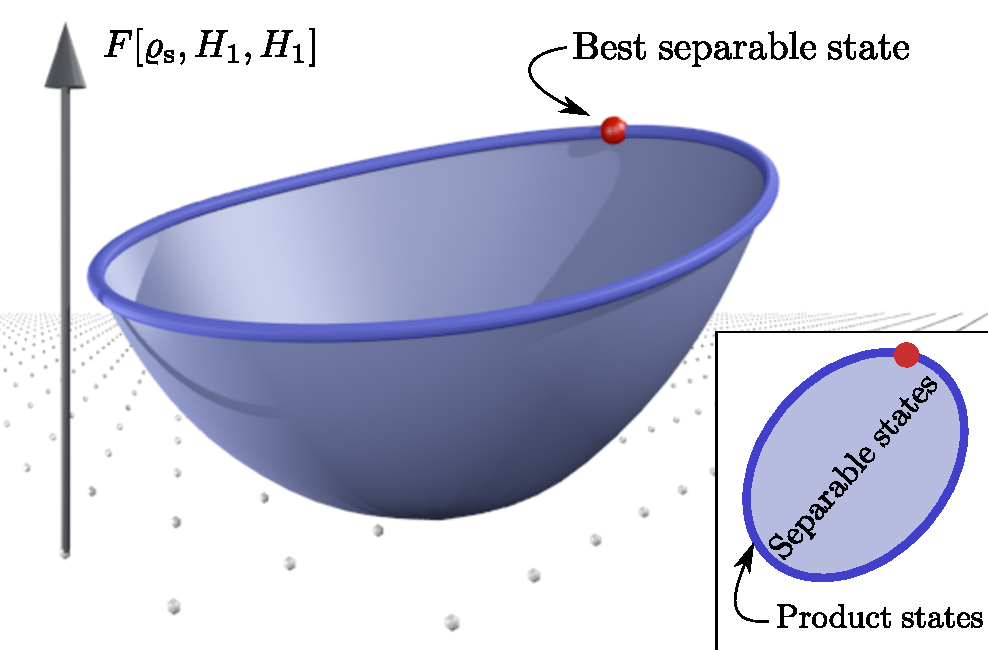
\includegraphics[width=244pt]{img/convex-function.pdf}
% \caption{Graphic representation of the separable states and the
% convexity of QFI. Blue dot takes the highest possible value.
% On the bottom right, we show the top view of the convex set of states
% where the states placed in the red border are the pure product states.}
% \label{fig:convexity in separable states of qfi}
% \end{center}
% \end{figure}

As we mentioned before, the best possible precision bound will be reached for a pure product state that maximises all $(\Delta j_z^{(n)})^2$.
From the definition of the variance,
\be
(\Delta j_z^{(n)})^2=
\expect{(j_z^{(n)})^2}-\expect{j_z^{(n)}}^2.
\ee
Hence, We try a state that approaches to zero its polarisation on the $OZ$ direction and maximises \expect{(j_z^{(n)})^2}.
We have that  $\ket{\psi}=(\ket{+j}+\ket{-j})/\sqrt{2}$ is ideal for this.
The inner state for all particles is just the product state $\rho_{\rm s} =\ket{\psi}\bra{\psi}^{\otimes N}$.
Notice that this state is permutationally invariant, hence it is a tight bound for what can be achieved with PI separable states.
The variance of a single particle operator is $(\Delta j_z^{(n)})^2=j^2$ so the proof holds.

After this discussion we make the following observation. The best achievable precision for separable states is written as
\be
(\Delta b_1)^{-2} \leq 4N j^2 \sigma^2,
\label{eq:best_separable}
\ee
where the state itself is sensitive to homogeneous fields.
This bound coincides with the totally polarized state studied before when the spin number $j$ is equal to half.
\label{obs:precision bound for separable states}

In the following we try to find a better precision bound making use of presumably better entangled states.
Note that the bound for the singlet state, even if it is entangled, is above the bound for the totally polarised state but below of the bound defined for the best separable state.
Nevertheless, when the singlet state is used effect of the homogeneous magnetic field has not to be compensated since it is insensitive to it and thus the bound can be saturated with an optimal estimator for the gradient field.

%%%%%%%%%%%%%%%%%%%%%%%
\ssssection{The unpolarised Dicke states $\ket{Nj, 0}$ and $\ket{Nj, 0}_x$}
%%%%%%%%%%%%%%%%%%%%%%%

Unpolarised Dicke states play an important role in quantum opticsand quantum information science.
The Dicke state $\ket{Nj,0}_l$ with a maximal $\langle J_x^2+J_y^2+J_z^2 \rangle$ and $\langle J_l\rangle=0$ for any $l\in x,y,z$ is particularly interesting due to its entanglement properties and its metrological usefulness.
This state has been created in photonic experiments \cite{Kiesel2007,Wieczorek2009,Chiuri2012} and in cold atoms \cite{Lucke2011,Hamley2012}, while a Dicke state with $\langle J_z\rangle>0$ has been created with cold trapped ions \cite{Haffner2005}.

The Dicke state $\ket{Nj, 0}$ is an eigenstate of $J_z$ so insensitive to homogeneous magnetic field pointing into the $OZ$ direction, thus the precision can be saturate by some measurement.
Whereas, The Dicke state $\ket{Nj, 0}_x$ is sensitive to the homogeneous field.
Moreover it is very useful for homogeneous magnetometry as it has been shown in Reference~[XXX].
Here we consider large particle numbers, to make the results simpler.

Since both Dicke states are pure, we have that
the QFI appearing on Equations~(\ref{eq:precision bound for single-cloud
systems IH}, \ref{eq:precision bound for single-cloud
systems SH}) are simply four times the following variances of $j_z^{(n)}$ and $J_z$.
Since both Dicke states are unpolarized, all the first moments $\expect{J_l}$ are equal to zero and due to they are PI all $\expect{j_l^{(n)}}$ are also zero for all $l\in x,y,z$.
Therefore, we only need to compute the second moments to compute the variances.


We will compute all the second moments on all directions of single particle operators $j_l^{(n)}$ as well as the global operators $J_l$ for $\ket{Nj,0}$.
Later on, we will map those result to the Dicke state for the $OX$ direction.
We have the following characteristic identities for $\ket{Nj,0}$, $\expect{J_z^2} = 0$ and $\expect{J_{\perp z}^2} = \frac{Nj(Nj+1)}{2}$ where "${\perp}{z}$" can be seen as $x$ or $y$.
From the global second moments we can write for the single particle the following,
\begin{align}
  \expect{(j_z^{(n)})^2} &= -(N-1)\expect{j_z^{(n)}j_z^{(m)}} \\
  \expect{(j_{\perp z}^{(n)})^2} &= \tfrac{j(Nj+1)}{2}-(N-1)\expect{j_{\perp z}^{(n)}j_{\perp z}^{(m)}}
\end{align}
for all $\forall n\neq m$ due to the PI nature of the state.
Together with $\expect{(j_z^{(n)})^2+2(j_{\perp z}^{(n)})^2} = j(j+1)$ due to the rotational symmetry on $OZ$, we have three independent equations relating all the four moments.
In Reference~\cite{Urizar-lanz2013}, a mapping between the Dicke states of spin-$j$ ensembles and of spin-$\frac{1}{2}$ ensembles was provided, by which the expectation value
\be
  \expect{(j_z^{(n)})^2}= \tfrac{(N-1)j^2}{2jN - 1}
\ee
was derived.
With this we are able to obtain all the rest unknown values we are searching for.
In the large $N$ limit, this gives
\be
\label{eq:jz2 for dicke state large number of particles}
\lim_{N \to \infty} \expect{(j_z^{(n)})^2}=\tfrac{j}{2}.
\ee
From Eq.~\eqref{eq:precision bound for single-cloud
systems IH} we can conclude that $\qfi[\rho_{\rm s},j_z^{(1)}]=2j$,
hence the proof for homogeneous insensitive $\ket{Nj,0}$ holds.

Now we have only to apply a mapping between the $OX$ and $OZ$ axis to obtain the respective second moments for $\ket{Nj,0}_{x}$.
We do that on the large $N$ limit,
\be
  \lim_{N \to \infty} \expect{(j_z^{(n)})^2}=\tfrac{j(2j+1)}{4}.
\ee
Finally, we have all the ingredients to go forward on writing the precision bound.

For large $N,$ the precision bound for the Dicke $\ket{Nj,0}$ state is
\be
\label{eq:exact precision bound for dicke ih state}
(\Delta b_1)^{-2}_{\max} =2Nj\lpar \sigma^2
-\eta\rpar,
\ee
whereas for the homogeneous sensitive Dicke state $\ket{Nj,0}_x$ the precision is bounded from above by
\be
(\Delta b_1)^{-2}\leq Nj(2j+1) (\sigma^2 -\eta)+ 2 Nj(Nj+1) \eta,
\ee
which shows in principle a Heisenberg behavior in the second term on
the right-hand side.
%
%
% %%%%%%%%%%%%%%%%%%%%%%%
% \subsubsection{The perpendicular Dicke state $\ket{Nj, 0}_x$}
% %%%%%%%%%%%%%%%%%%%%%%%
%
% The perpendicular Dicke state is
% a highly entangled state, which is very useful for homogeneous magnetometry.
% This is a consequence of the fact that the variance of the $J_z$ operator
% scales with $N^2$,  more concretely $ \expect{J_z^2}=Nj(Nj+1)/2$. This can be derived from
% \be
% \expect{\bs{J}^2} = \expect{J_y^2} +\expect{J_z^{2}} = Nj(Nj+1),
% \ee
% by taking into account that, due to
% rotational symmetry along the $x$-axis, $\expect{J_y^2}$ and $\expect{J_z^2}$ are
% equal.
%
% Let us now investigate the perpendicular Dicke state from the point of view of
% gradient magnetometry.
% To calculate the corresponding QFI, we need to
% determine the $\expect{(j_z^{(1)})^2}$ expectation value.
% The axial-symmetry of $\ket{Nj, 0}_x$ implies that
% \be
% \expect{(j_x^{(1)})^2}+2\expect{(j_z^{(1)})^2}=j(j+1).
% \ee
% Using the result obtained in Eq.~(\ref{eq:jz2
% for dicke state large number of particles}), with a trivial
% $x\leftrightarrow z$ mapping,
% we know that $\expect{(j_x^{(1)})^2}=\tfrac{j}{2}$ for large $N$, thus
% \be
% \expect{(j_z^{(1)})^2}=\frac{j(2j+1)}{4}.
% \ee
% Then using Eq.~(\ref{eq:precision bound for single-cloud systems
% SH}) and noting that $\qfi[\rho_{\rm s},
% j_z^{(1)},j_z^{(1)}]=4\expect{(j_z^{(1)})^2}$ and  $\qfi[\rho_{\rm s},
% J_z,J_z]=4\expect{J_z^2}$ hold for pure states with
% $\expect{(j_z^{(1)})}=\expect{J_z}=0$, we arrive at the following result for
% the precision bound of the perpendicular Dicke state for a large number of
% particles
%
%
% % As we are left with
% %that with perpendicular Dicke states one may in principle reach
% %the Heisenberg limit for gradient magnetrometry will require a more
% %deep.
%
%

%%%%%%%%%%%%%%%%%%%%%%%
\ssssection{The GHZ state}
%%%%%%%%%%%%%%%%%%%%%%%

The Greenberger-Horne-Zeilinger (GHZ) states are also highly entangled states that play an important role in quantum physics \cite{Greenberger1990}.
They have been created experimentally in photonic systems \cite{Pan2000,Yao2012,Lu2007} and trapped ions \cite{Sacket2000,Monz2011}.

The GHZ state is defined for qubits in the following way
\be
\label{eq:definition of ghz}
\ket{{\rm GHZ}} = \tfrac{1}{\sqrt{2}}(\ket{0\cdots0}+\ket{1\cdots1}).
\ee
This state is very sensitive to the homogeneous field.
On the other hand, as shown in Appendix~\ref{app: the ghz state saturable}, for this state the optimal estimators for the homogeneous field and the gradient field are compatible.
It means that both parameters can be estimated at once.
Hence, in this case, the bound given in Eq.~(\ref{eq:precision bound for single-cloud systems SH}) can be saturated by some measurement set-up.
In order to calculate this bound explicitly, let us recall that for pure states the QFI is simplified to Eq.~\eqref{eq:QFI_pure}.
In the GHZ state the expectation value of $j_z^{(n)}$ and
$J_z$ is equal to zero, as it was for the Dicke state, and $\expect{(j_z^{(n)})^2}=j^2$ and $\expect{J_z^2}
= N^2j^2$, hence we obtain the following result
\be
\label{eq:precision bound for ghz}
(\Delta b_1)^{-2}_{\max} = 4Nj^2\sigma^2 +4N(N-1)j^2\eta.
\ee
This means that we can reach the Heisenberg-limit with such states, but only in
cases where $\eta$ is positive\ie that the particles stay spatially correlated.

%%%%%%%%%%%%%%%%%%%%%%%
\ssssection{Summary of results}
%%%%%%%%%%%%%%%%%%%%%%%

Finally, we summarise the precision bounds obtained for various quantum states in Table~\ref{tab:compare all the states}.
In Fig.~{\ref{fig:different states}}, we show the mean values and variances
of the collective angular momentum components for these states.

\begin{figure}[htp]
\begin{center}
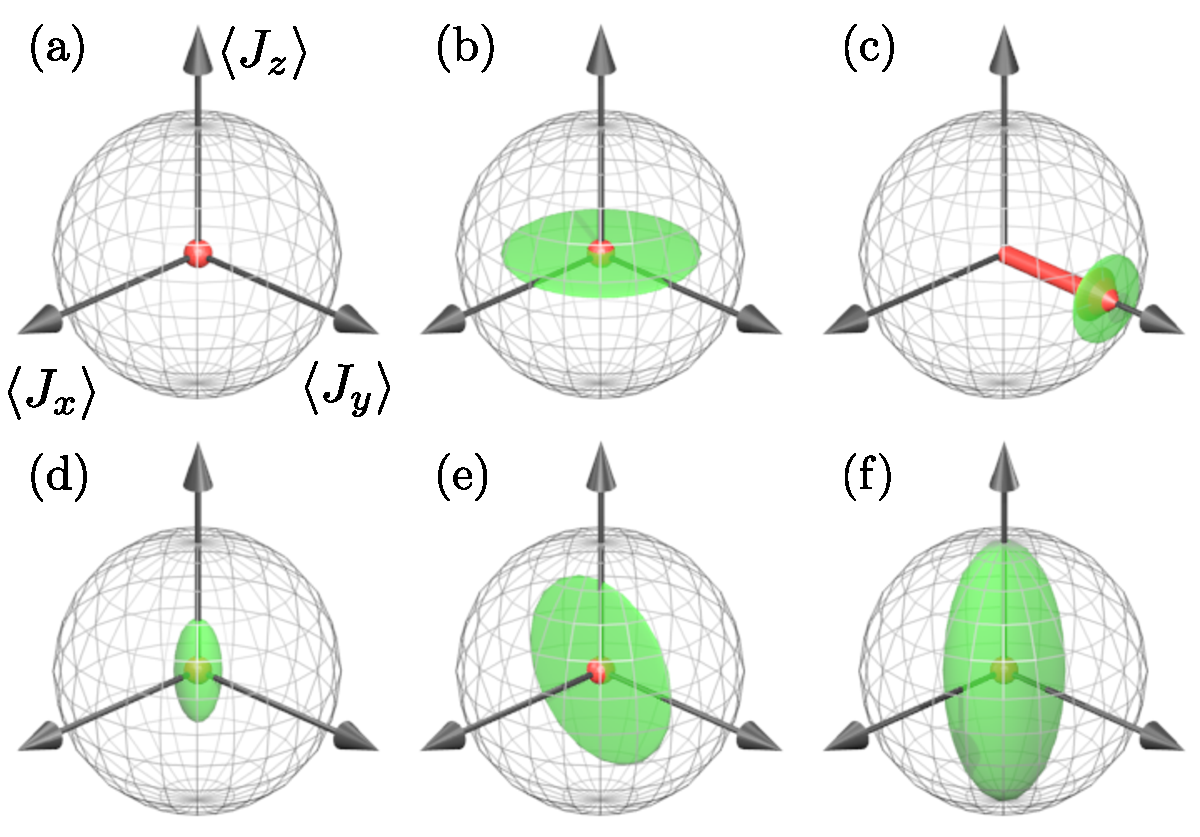
\includegraphics[width=244pt]{img/states-representation.pdf}
\caption{Angular momentum components and their variances for various quantum states.
The mean value of the collective angular momentum $\bs{J}$ is represented by a
red dot or arrow.
The radius of the sphere is the maximal angular momentum, $r=Nj$.
The green uncertainty ellipses describe the uncertainties of the spin components.
%The green volume represents the variance in each direction, the more the
%width of the ellipsoid the more the variance in that direction.
In this case are represented different states for few particles
due to the different scaling of the variances in terms of $N$, namely,
singlet states (a), Dicke state (b), totally polarised state (c),
best separable state (d), perpendicular Dicke state (e), and the GHZ (f).}
\label{fig:different states}
\end{center}
\end{figure}

\begin{table}
  \begin{center}
\begin{tabular}{|l|c|}
\hline
Singlet states& $(\Delta b_1)^{-2}|_{\max} =
\tfrac{4Nj(j+1)}{3}\lpar\sigma^2-\eta\rpar $\\
\hline
Totally polarised state & $(\Delta b_1)^{-2}\leq 2N
\sigma^2 j$ \\
\hline
Best separable state & $(\Delta b_1)^{-2} \leq 4N
\sigma^2 j^2$ \\
\hline
$\ket{Nj,0}$ Dicke state & $(\Delta b_1)^{-2}|_{\max} =\tfrac{Nj}{2}\lpar
\sigma^2-\eta\rpar$\\
\hline
$\ket{Nj,0}_{x}$ Dicke state & $(\Delta b_1)^{-2}\leq
N(\sigma^2 -\eta)(2j^2+j)+ 2\eta Nj(Nj+1)$ \\
\hline
GHZ state & $(\Delta b_1)^{-2}|_{\max} = 4Nj^2(\sigma^2 +(N-1)\eta)$ \\
\hline
\end{tabular}
\end{center}
\caption{Precision bounds for  differential
magnetometry for various quantum states.
For the definition of the states, see the text.
If the bound are proved to be saturable then
the \"max\" subscript is used instead of an inequality.}
\label{tab:compare all the states}
\end{table}
